\chapter{Measurable functions}
Throughout this chapter, let $(X, \Sigma)$ be a measurable space and let $B$ be a Banach space.
We would like to consider functions $f: X \to B$ which ``respect'' $\Sigma$. Then, given a measure $\mu$ defined on $\Sigma$, we will be able to define the integral $\int_{X} f~d\mu$ of $f$ with respect to $\mu$.

\section{Simple functions}
When we prove a theorem $T$ about functions in measure theory, we want to follow the following template:
\begin{enumerate}
\item Let $\mathcal F$ be the set of functions for which $T$ is true. Show that $\mathcal F$ contains all functions which are ``sufficiently simple.''
\item Show that $\mathcal F$ is closed under linear combination, so is a vector space.
\item Show that $\mathcal F$ is closed under taking limits of appropriate type.
\item Conclude that every appropriate function lies in $\mathcal F$.
\end{enumerate}
In this section we treat the ``sufficiently simple'' functions.

\begin{definition}
A \dfn{simple function} is a function $f: X \to B$ such that the image of $f$ is finite, and for every $b$ in the image of $f$, $f^{-1}(b)$ is a measurable set.
The set of simple functions is denoted $\Simp(X \to B)$.
\end{definition}

\begin{subsec}
The simple functions have a particularly convenient canonical form.
To define them, we first characterize the $\RR$-valued simple functions.
\end{subsec}

\begin{definition}
Let $Y \subseteq X$ be a measurable set. The \dfn{indicator function} of $Y$, denoted $1_{Y}$, is the function $X \to \{0, 1\}$, defined by $1_{Y}(y) = 1$ if $y \in Y$ and $1_{Y}(y) = 0$ if $y \notin Y$.
\end{definition}

\begin{subsec}
Note that every indicator function is simple, since its image is $\{0, 1\}$, the preimage of $0$ is $Y^{c}$, the preimage of $1$ is $Y$, and $Y,Y^{c}$ are both measurable.
Conversely, if $f \in \Simp(X \to \CC)$, $f$ is a linear combination of indicator functions. In fact, if $\{y_{1}, \dots, y_{n}\}$ is the image of $f$, and the preimage of $y_{i}$ is $Y_{i}$, then
\[f(x) = \sum_{i=1}^{n} y_{i}1_{Y_{i}}(x).\]
Indeed, the $Y_{i}$ are disjoint since they are preimages of distinct real numbers, so $y_{i}1_{Y_{i}}(x) = y_{i}$ iff $f(x) = y_{i}$, and $f(x) = 0$ otherwise.
This characterization also works for $B$-valued simple functions: if $\{b_{1}, \dots, b_{n}\}$ is the image of $f$, and the preimage of $b_{i}$ is $Y_{i}$, then
\[f(x) = \sum_{i=1}^{n} b_{i}1_{Y_{i}}(x).\]
\end{subsec}

\begin{subsec}
We now show that $\Simp(X \to B)$ is closed under various operations.
\end{subsec}

\begin{definition}
A vector space $A$ over $\CC$ is called an \dfn{algebra} if it is equipped with a multiplication $A \times A \to A$ which is associative, distributes over addition, and satisfies, for every $c,d \in \CC$ and $x,y \in A$,
\[(cx)(dy) = (cd)(xy).\]
If the multiplication of $A$ has an identity, we call the identity $1$ and call $A$ a \dfn{unital algebra}.
\end{definition}

\begin{subsec}
In particular, a collection of functions is an algebra iff it is closed under multiplication.
See Exercise~\ref{algebra review}.
\end{subsec}

\begin{lemma}\label{Simp is an algebra}
$\Simp(X \to B)$ is a vector space. In particular, $\Simp(X \to \CC)$ is a unital algebra.
\end{lemma}
\begin{proof}
Let $f, g \in \Simp(X \to B)$, say
\[f(x) = \sum_{i=1}^{n} y_{i}1_{Y_{i}}(x)\]
and
\[g(x) = \sum_{j=1}^{m} z_{j}1_{Z_{j}}(x).\]
We first claim that $f + g$ is simple. In fact, the image of $f + g$ is contained in $\{y_{i} + z_{j}: 1 \leq i \leq n, ~1 \leq j \leq m\}$, and the preimage of $y_{i} + z_{j}$ under $f + g$ is $Y_{i} \cap Z_{j}$.

The proof that $\Simp(X \to B)$ is closed under scaling is similar. Clearly $\Simp(X \to B)$ is nonempty, so this implies that $\Simp(X \to B)$ is a vector space.

Now if $B = \CC$, function multiplication is defined, and
\[fg(x) = \sum_{i=1}^{n} y_{i}1_{Y_{i}}(x)\sum_{j=1}^{m} z_{j}1_{Z_{j}}(x) = \sum_{i,j} y_{i}z_{j} 1_{Y_{i} \cap Z_{j}}(x).\]
Therefore $fg$ is simple.
Moreover, the function $f(x) = 1$ is an identity for multiplication.
\end{proof}

\begin{lemma}\label{Simp is closed under minmax}
Let $f, g \in \Simp(X \to \CC)$. Then $|f| \in \Simp(X \to \CC)$. In fact, if $f, g \in \Simp(X \to \RR)$, then $\max(f, g) \in \Simp(X \to \RR)$ and $\min(f, g) \in \Simp(X \to \RR)$.

Moreover, if $f \in \Simp(X \to B)$, the function $x \mapsto ||f(x)||$ is in $\Simp(X \to \CC)$.
\end{lemma}
\begin{proof}
Left as Exercise~\ref{Simp closure exer}.
\end{proof}

\begin{exercise}\label{algebra review}
Look up or prove the following algebraic theorems:
\begin{enumerate}
\item Let $\varphi: \CC \to A$ be a morphism of rings. Then $A$ is an algebra, where scalar multiplication is defined by $za = \varphi(z)a$, for any $z \in \CC$ and $a \in A$. We call $\varphi$ the \dfn{canonical inclusion} of $\CC$ into $A$.
\item If $A$ is a unital algebra with multiplicative identity $1_{A}$, then the map $\varphi(z) = 1_{A}z$, $\varphi: \CC \to A$, is a morphism of rings, and is in fact the canonical inclusion of $\CC$ into $A$.
\item If $V$ is a vector space of functions $X \to \CC$, then $V$ is an algebra over $\CC$ iff $V$ is closed under function multiplication.
\end{enumerate}
None of these theorems actually require that we are working over $\CC$; they are valid if $\CC$ is replaced with any field.
However, you are not expected to check that.
\end{exercise}

\begin{exercise}\label{Simp closure exer}
Prove Lemma~\ref{Simp is closed under minmax}.
\end{exercise}

\begin{exercise}\label{Borel-Cantelli}
If ${(A_{n})}_{n}$ is a sequence of measurable sets, we define $\limsup_{n \to \infty} A_{n}$ by the relation
\[1_{\limsup_{n \to \infty} A_{n}} = \limsup_{n \to \infty} 1_{A_{n}}.\]
Then:
\begin{enumerate}
\item Show that $\limsup_{n \to \infty} A_{n}$ is a well-defined measurable set.
\item Show that $x \in \limsup_{n \to \infty} A_{n}$ iff there are infinitely many $n \in \NN$ such that $x \in A_{n}$.
\item Prove the \dfn{Borel-Cantelli lemma}: If $\mu$ is a nonnegative measure on $X$ such that
\[\sum_{n=1}^{\infty} \mu(A_{n}) < \infty,\]
then $\limsup_{n \to \infty} A_{n}$ is $\mu$-null.
\end{enumerate}
The Borel-Cantelli lemma is a primitive example of a ``zero-one law'', a theorem that implies that certain sets must either be null or have null complement.
\end{exercise}

\begin{exercise}
Given $x \in [0, 1)$, we may assign $x$ a canonical decimal expansion by not letting $x$ have a decimal expansion that ends with an infinitely repeating string of nines.
We let $x_{j} \in \{0, \dots, 9\}$ denote the $j$th entry in the canonical decimal expansion of $x$ (so for example ${(\pi - 3)}_{3} = 1$).
Let us say that $x$ has \dfn{uniform expansion} at $n \in \NN$ if for every $d \in \{0, \dots, 9\}$, the set of $j \in \{1, \dots, 10n\}$ such that $x_{j} = d$ has cardinality $n$.
In other words, $x$ has uniform expansion at $n$ iff for every $d \in \{0, \dots, 9\}$ the probability that a $j \in \{1, \dots, 10n\}$ drawn uniformly at random satisfies $x_{j} = d$ is $1/10$.

Let $A$ be the set of $x \in [0, 1)$ such that there are infinitely many $n \in \NN$ such that $x$ has uniform expansion at $n$.
Show that $A$ is a Borel set, and that $A$ is Lebesgue null. (Hint: Use the Borel-Cantelli lemma, Exercise~\ref{Borel-Cantelli}).)
\end{exercise}



\section{Measurable functions}
We want to know which functions $X \to B$ are ``good'' from the perspective of measure theory. To accomplish this, recall the notion of pointwise convergence.

\begin{definition}
A sequence of functions $f_{n}: X \to B$ is said to \dfn{converge pointwise} to a function $f$ if for every $x \in X$,
\[f(x) = \lim_{n \to \infty} f_{n}(x).\]
\end{definition}

\begin{subsec}
Let $\mu$ be a complete measure on $\Sigma$.
If $\mu$ is not already complete, we can always expand $\Sigma$ by adjoining the $\mu$-null sets to $\Sigma$, so this assumption is no loss in generality.
\end{subsec}

\begin{subsec}
In measure theory, a property is said to hold \dfn{almost everywhere} if it holds everywhere except a null set, and hold \dfn{almost nowhere} if it only holds on a null set.
We will refer to measurable functions whose definition only makes sense almost everywhere as if they were defined on all of $X$.
\end{subsec}

\begin{example}
Let $\mu$ be Lebsegue measure on $\RR$ and $f(x) = 1/x$.
Then $f(0)$ is not defined, but $\{0\}$ is a $\mu$-null set.
So we can view $f$ as a function $\RR \to \CC$, even though it is only defined almost everywhere.
\end{example}

\begin{subsec}
Because $\mu$-null sets are not very important, we want to view two functions that are equal almost everywhere as actually being the same function, modulo ``measurement error''.
For example, if $u(x)$ denotes the temperature in the air at a point $x \in \RR^{3}$ measured by some thermometer, and we measure that $u(x) = 0$ at every $x$ close to $0$, but $u(0) = 1$, then we must have made an error in the measurement of $u(0)$, and might as well view this measurement $u$ as ``the same as'' the measurement of temperature which is identically $0$ in a neighborhood of $0$.
\end{subsec}

\begin{definition}\label{almost converge dfn}
Let $\mu$ be a measure on $\Sigma$. A sequence of functions $f_{n}: X \to B$ is said to \dfn{converge pointwise almost everywhere} with respect to $\mu$, or simply \dfn{almost converge}, to a function $f: X \to B$ if there is a null set $Z$ such that on $X \setminus Z$, $f_{n} \to f$ pointwise. In this case, we write
\[f = \lim_{n \to \infty} f_{n},\]
noting that the limit is meant almost everywhere if unclear from context.
\end{definition}

\begin{subsec}
Note that in Definition~\ref{almost converge dfn}, we allow the functions $f_{n}$, or their limit $f$, to be undefined on a null set, which is then viewed as a subset of the bad set $Z$ where the $f_{n}$ may not converge to $f$.
\end{subsec}

\begin{example}
Any sequence of functions which converges pointwise almost converges.
As an example of a sequence of functions which almost converges but doesn't converge pointwise, let $f_{n}(x) = x^{n}$, $X = [0, 1]$. Then $f_{n} \to 0$ everywhere except $1$, so $f_{n} \to 0$ almost everywhere with respect to Lebesgue measure.
\end{example}

\begin{definition}
A \dfn{measurable function} $f: X \to B$ is a function such that there is a sequence $f_{n} \in \Simp(X \to B)$ such that $f_{n} \to f$ almost everywhere.
Let $\mathcal M(X \to B)$ denote the set of measurable functions.
\end{definition}

\begin{subsec}
The notation $\mathcal M(X \to B)$ will make more sense when we define the $L^{p}$-spaces later on.
We will abuse notation and write $\mathcal M$ if $X,B$ are clear from context, and may also write something like $\mathcal M(X \to B, \mu)$ if $\mu$ is not clear from context.
\end{subsec}

\begin{lemma}
$\mathcal M(X \to B)$ is a vector space.
In particular, $\mathcal M(X \to \CC)$ is an algebra such that if $f, g \in \mathcal M(X \to \CC)$, then so are $\max(f,g)$, $\min(f,g)$, and $|f|$.
Moreover, if $f \in \mathcal M(X \to B)$, then $x \mapsto ||f(x)||$ is in $\mathcal M(X \to \CC)$.
\end{lemma}
\begin{proof}
Let $f,g \in \mathcal M(X \to B)$, and suppose that $f_{n} \in \Simp(X \to B)$, $f_{n} \to f$. Similarly let $g_{n} \to g$, $g_{n} \in \Simp(X \to B)$.
Then $f_{n} + g_{n} \in \Simp(X \to B)$ by Lemma~\ref{Simp is an algebra} and $f_{n} + g_{n} \to f + g$.

We leave the other claims as an exercise for the reader.
\end{proof}

\begin{subsec}
Let $N$ be the set of all functions $f$ which are zero almost everywhere, thus there is a null set $Z$ such that on $X \setminus Z$, $f = 0$.
\end{subsec}

\begin{lemma}
The set $N$ of functions that are zero almost everywhere is a vector subspace of $\mathcal M(X \to B)$.
\end{lemma}
\begin{proof}
Let $f \in N$, and suppose that $Z$ is the set where $f$ is nonzero.
We first claim that $f$ is measurable; in fact, the sequence $f_{n} = 0$ converges to $f$ pointwise except on $Z$, hence almost everywhere.

Now if $g \in N$, and $g$ is nonzero on a set $W$, then $f + g$ is nonzero on a subset of the null set $Z \cup W$; since $\mu$ is complete, any subset of $Z \cup W$ is null. The argument for scalars is similar. Clearly $0 \in N$ so $N$ is nonempty.
\end{proof}

\begin{subsec}
Whenever $W$ is a vector subspace of a vector space $V$, we may form its quotient space $V/W$ of equivalence classes, where two elements $f, g \in V$ are viewed as equivalent if $f - g \in W$.
In particular, if we take the quotient $\mathcal M(X \to B)/N$, two functions $f,g$ are equivalent iff $f - g$ is zero almost everywhere.
\end{subsec}

\begin{definition}
Let $N$ be the space of all functions that are zero almost everywhere is a vector subspace. We denote its quotient space
\[M(X \to B) = \frac{\mathcal M(X \to B)}{N}.\]
We will abuse terminology and refer to equivalence classes $f \in M(X \to B)$ as ``functions'', and a representative of an equivalence class $f$ as a \dfn{version} of $f$.
\end{definition}

\begin{subsec}
Again, we may write $M(X \to B, \mu)$ and similar notations to mean $M(X \to B)$.
In general, we will want to work with $M$ whenever possible rather than $\mathcal M$.
\end{subsec}

\begin{exercise}
Let $\mu$ be a probability measure on a measurable space $X$.
Let ${(f_{n})}_{n}$ be a sequence of measurable functions on $(X, \mu)$, and $f$ a measurable function on $(X, \mu)$.
Assume that for every $\varepsilon > 0$, one has
\[\sum_{n=1}^{\infty} \mu(\{x \in X: ||f_{n}(x) - f(x)|| > \varepsilon\}) < \infty.\]
Show that $f_{n} \to f$ almost everywhere.

This characterization is highly useful in probability, where one is typically not able to refer directly to elements of $X$, but only measurable sets, but still wants to be able to discuss convergence almost everywhere.
(Hint: Use the Borel-Cantelli lemma, Exercise~\ref{Borel-Cantelli}).)
\end{exercise}



\section{Characterizing measurable functions}
The current definition of $M$ is unwieldly. Its elements are equivalence classes of functions, themselves defined to be the limits of simple functions, whose definition was natural but already little long.
Here we give another characterization of measurability that is somewhat easier to work with, and will readily imply that every function that is relevant to analysis is measurable.

\begin{subsec}
Throughout, we as usual fix a complete measured space $(X, \Sigma, \mu)$ and a Banach space $B$.
\end{subsec}

\begin{definition}\label{almost separably valued dfn}
A function $f: X \to B$ is \dfn{almost separably valued} if there is a null set $Z$ such that $f(X \setminus Z)$ is separable in the topology of $B$.
\end{definition}

\begin{subsec}
Being almost separably valued is a good condition. It means that, modulo a harmless null set, the image of $f$ consists of points which can be approximated by points that lie in a countable set $C$; and elements of $C$ then are likely to admit finitary descriptions.
Think of how difficult $\RR$ would be to work with if we did not have $\QQ$, whose elements are described as pairs of natural numbers!
\end{subsec}

\begin{subsec}
Thankfully, most Banach spaces that arise naturally in analysis turn out to be separable; certainly any finite-dimensional vector space has this property, and all but one Banach space that we will consider in this text will be separable.
Certainly any function into a separable Banach space is almost separably valued. So Definition~\ref{almost separably valued dfn} will turn out to be a slightly annoying technical condition, and not at all of import, in practice.
The reader who is only interested in the case $B = \CC$, which is reasonable to do on one's first reading, can forget about this hypothesis altogether.
\end{subsec}

\begin{definition}
The \dfn{carrier}\footnote{Some books prefer the term ``support'', but we use ``support'' to mean the closure of the carrier, whenever $(X, \mu)$ has a topology.} of a function $f: X \to B$ is the set $\{x \in X: f(x) \neq 0\}$.
\end{definition}

\begin{subsec}
Now $B$ has a norm, so it has open balls $B(x, r) = \{y \in B: ||x - y|| < r\}$, and in particular $B$ has a topology: its open sets are the unions of the balls $B(x, r)$.
So we can define its Borel $\sigma$-algebra in the usual way: it is the smallest $\sigma$-algebra containing the topology of $B$.
\end{subsec}

\begin{subsec}
Our goal in this section is to prove the following theorem:
\end{subsec}

\begin{theorem}\label{characterization of measurable functions}
Let $f: X \to B$ be a function with carrier $C$, possibly only defined almost everywhere. Then the following are equivalent:
\begin{enumerate}
\item $f$ is measurable.
\item $f$ is almost separably valued and for every open set $U \subseteq B$, $f^{-1}(U) \cap C$ is measurable.
\item $f$ is almost separably valued and for every closed set $K \subseteq B$, $f^{-1}(K) \cap C$ is measurable.
\item $f$ is almost separably valued and for every Borel set $W \subseteq B$, $f^{-1}(W) \cap C$ is measurable.
\end{enumerate}
\end{theorem}

\begin{corollary}\label{characterization of measurable functions II}
Let $\Gamma$ be the Borel $\sigma$-algebra of $B$, so $B = (B, \Gamma)$ is a measurable space whose measurable sets are exactly the Borel sets.
Then a function $f: X \to B$ is measurable iff $f$ is almost separably valued and for every measurable $Y \subseteq B$, $f^{-1}(Y)$ is measurable.
\end{corollary}

\begin{subsec}
The reader should compare Corollary~\ref{characterization of measurable functions II} to the result which says that a function $f$ is continuous iff the preimage of an open set is open. It says that a measurable function $X \to B$ is, modulo sets of measure zero, the same thing as a measurable map $X \to B$, where $B$ is equipped with its Borel $\sigma$-algebra.
\end{subsec}

\begin{subsec}
Before we prove Theorem~\ref{characterization of measurable functions}, we need several lemmata which are useful in their own right.
\end{subsec}

\begin{lemma}\label{Newberger lemma 1}
Let $f_{n}: X \to B$ be a sequence of functions converging pointwise to a function $f$.
For every open $U \subseteq B$, we define $U_{n} = \{y \in U: \inf_{x \notin U} ||x - y|| > 1/n\}$.
Then
\[f^{-1}(U) = \bigcup_{n=1}^{\infty} \bigcup_{K=1}^{\infty} \bigcap_{k=K}^{\infty} f_{k}^{-1}(U_{n}).\]
\end{lemma}
TODO:\@ Draw a picture of $U_{n}$
\begin{proof}
The following are equivalent:
\begin{enumerate}
\item $x \in f^{-1}(U)$.
\item $f(x) \in U$.
\item There are $n, K$ such that for every $k \geq K$, $f_{k}(x) \in U_{n}$.
\item There are $n, K$ such that for every $k \geq K$, $x \in f_{k}^{-1}(U_{n})$.
\item There are $n, K$ such that $x \in \bigcap_{k \geq K} f_{k}^{-1}(U_{n})$.
\item $x \in \bigcup_{n} \bigcup_{K} \bigcap_{k \geq K} f_{k}^{-1}(U_{n})$.
\end{enumerate}
Indeed, for every $i \in \{1, \dots, 6\}$, the $i$th entry in the above list is clearly equivalent to the $i+1$th entry.
\end{proof}

\begin{definition}
A function $f: X \to B$ is \dfn{separably valued} if the image of $f$ is separable in $B$.
\end{definition}

\begin{lemma}\label{Newberger lemma 2}
Let $f: X \to B$ be a function with carrier $C$. Then the following are equivalent:
\begin{enumerate}
\item $f$ is the pointwise limit of simple functions.
\item $f$ is separably valued and for every open set $U \subseteq B$, $f^{-1}(U) \cap C$ is measurable.
\item $f$ is separably valued and for every open ball $U \subseteq B$, $f^{-1}(U) \cap C$ is measurable.
\end{enumerate}
\end{lemma}
\begin{proof}
We first show that $1$ implies $2$.
Let $f_{n} \to f$ pointwise, $f_{n} \in \Simp(X \to B)$ and for every $n$, let $\{b_{1}^{n}, \dots, b_{k(n)}^{n}\}$ be the image of $f_{n}$.
Let $K$ be the closure of $K_{0} = \{b_{i}^{n}: n \in \NN,~i \in \{1, \dots, k(n)\}\}$.
Then $K_{0}$ is countable and dense in $K$, so $K$ is separable; moreover, $f(X) \subseteq K$, so $f$ is separably valued.
Now let $U \subseteq B$ be an open set; then $f^{-1}(U) \cap C = f^{-1}(U \setminus \{0\})$, and $U \setminus \{0\}$ is open.

Thus we must show that if $V$ is an open set which does not contain $0$, $f^{-1}(V)$ is measurable. Let $V_{k} = \{y \in V: \inf_{x \notin V} ||x - y|| > 1/n\}$. Clearly $f_{n}^{-1}(V_{k})$ is measurable since there are only finitely many points of $f_{n}(X)$ in $V_{k}$, each with a measurable preimage, and Lemma~\ref{Newberger lemma 1} implies
\[f^{-1}(V) = \bigcup_{n=1}^{\infty} \bigcup_{K=1}^{\infty} \bigcap_{k=K}^{\infty} f_{k}^{-1}(V_{n})\]
which is measurable since the measurable sets form a $\sigma$-algebra.

Clearly $2$ implies $3$ so it suffices to show that $3$ implies $1$.
Let $\{b_{i}: i \in \NN\}$ be dense in $f(X)$.
Let
\[C_{ij} = \{x \in C: ||f(x) - b_{i}|| < 1/j\}.\]
Then $C_{ij}$ is a preimage of a union of open balls, so $C_{ij}$ is measurable.
Now it would be reasonable to define for every $x \in C_{ij}$, $f_{n}(x) = b_{i}$, except that the $C_{ij}$ are not disjoint.

To rectify this problem, let
\[E_{ijn} = C_{ij} \setminus \bigcup_{\substack{(i,j) < (k, \ell) \leq (n, n)\\1 \leq i,j \leq n}} C_{k\ell}\]
where $(i, j) \leq (k, \ell)$ iff $j < \ell$ or $j = \ell$ and $i \leq k$.
Then if $n$ is fixed, the $E_{ijn}$ are disjoint, $E_{ijn} \subseteq C_{ij}$.
Now let
\[f_{n} = \sum_{i,j=1}^{n} b_{i} 1_{E_{ijn}}.\]
\begin{sublemma}
$f_{n} \to f$ pointwise.
\end{sublemma}
\begin{proof}
Let $x \in X$. If $f(x) = 0$, then for every $n$, $f_{n}(x) = 0$, so $f_{n}(x) \to f(x)$.

Otherwise, $x \in C$. Let $\varepsilon > 0$. Let $N_{1} > 1/\varepsilon$ and choose $N_{2}$ so that
\[||f(x) - b_{N_{2}}|| < \frac{1}{N_{1}}.\]
Now let $N = \max(N_{1}, N_{2})$. Then $x \in C_{N_{2}N_{1}}$, so if $n > N$,
\[(k, \ell) = \max_{(N_{1}, N_{2}) \leq (i, j) \leq (n, n)} (i,j),\]
then $x \in E_{k\ell n}$. Therefore $f_{n}(x) = b_{k}$ and
\[||f(x) - b_{k}|| < \frac{1}{\ell} \leq \frac{1}{N_{1}} < \varepsilon.\]
But $f_{n}(x) = b_{k}$, so $||f_{n}(x) - f(x)|| < \varepsilon$.
\end{proof}
This implies $1$.
\end{proof}

\begin{lemma}\label{Newberger lemma 3}
Let $f: X \to B$ be a function with carrier $C$. The following are equivalent:
\begin{enumerate}
\item For every closed set $K \subseteq B$, $f^{-1}(K) \cap C$ is measurable.
\item For every open set $U \subseteq B$, $f^{-1}(U) \cap C$ is measurable.
\item For every Borel set $W \subseteq B$, $f^{-1}(W) \cap C$ is measurable.
\end{enumerate}
\end{lemma}
\begin{proof}
Obviously $3$ implies $1$.

Now assume $1$. Then let $U \subseteq B$ be open,
\[K_{n} = \{y \in B: \inf_{x \notin U} ||x - y|| \geq \frac{1}{n}\}.\]
Then $K_{n}$ is closed and $U = \bigcup_{n} K_{n}$. But $f^{-1}(U) \cap C = \bigcup_{n} f^{-1}(K_{n}) \cap C$, and the $f^{-1}(K_{n}) \cap C$ are measurable, so $2$ follows.

To see that $2$ implies $3$, note that the set $\Gamma$ of all sets $Y$ such that $f^{-1}(Y) \cap C$ is measurable is a $\sigma$-algebra.
Indeed $\Gamma$ contains $\emptyset$ so is nonempty, is closed under complement since $f^{-1}(B \setminus Y) = X \setminus f^{-1}(Y)$, and is closed under countable union since $f^{-1}(\bigcup_{n} Y_{n}) = \bigcup_{n} f^{-1}(Y_{n})$.
Since $\Gamma$ contains the open sets, $\Gamma$ contains the Borel sets.
\end{proof}

\begin{proof}[Proof of Theorem~\ref{characterization of measurable functions}]
We can show that $f$ is measurable iff $f$ is almost separably valued and for every open set $U$, $f^{-1}(U) \cap C$ is measurable.
In fact, Lemma\label{Newberger lemma 3} then immediately shows that for every open set $U$, $f^{-1}(U) \cap C$ is measurable iff the same is true when ``open set'' is replaced with ``closed set'' or ``Borel set''.

First assume that $f$ is measurable. Then there are $f_{n} \in \Simp(X \to B)$ and a null set $Z$ such that $f_{n} \to f$ pointwise on $X \setminus Z$ and $f$ is defined on $X \setminus Z$.
So $f_{n}1_{X \setminus Z} \to f1_{X \setminus Z}$ (where $f1_{X \setminus Z} = 0$ if $f$ is undefined), so $f1_{X \setminus Z}$ meets the criteria of Lemma~\ref{Newberger lemma 2}; since null sets are measurable, so does $f$.

Conversely, if $Z$ is a null set such that $f(X \setminus Z)$ is separable and for every open set $U$, $f^{-1}(U) \cap C$ is measurable, then $f1_{X \setminus Z}$ is separably valued and for every open set $U$, ${(f1_{X \setminus Z})}^{-1}(U) \cap C$ is measurable, so Lemma~\ref{Newberger lemma 2} implies the claim.
\end{proof}

We now prove a very important theorem about measurable functions. Note that the analogous result for continuous functions (or even Riemann integrable functions) does not hold.

\begin{theorem}\label{measurable functions converge}
Suppose that $f_{n}$ are measurable functions which almost converge to a function $f$. Then $f$ is measurable.
\end{theorem}
\begin{proof}
We apply Newberger's theorem.
Since the $f_{n}$ are almost separably valued, there are null sets $Z_{n}$ such that $K = \overline{\bigcup_{n} f_{n}(X \setminus Z_{n})}$ is closed.
Therefore $f$ is almost separably valued. Then Lemma~\ref{Newberger lemma 1} implies that for every open set $U \subseteq B$,
\[f^{-1}(U) \cap C = \bigcup_{n=1}^{\infty} \bigcup_{K=1}^{\infty} \bigcup_{k=K}^{\infty} f_{n}^{-1}(U_{n}) \cap C\]
which implies that $f^{-1}(U)$ is a countable union of countable unions of countable intersections of measurable sets, hence is measurable.
\end{proof}

\begin{figure}
\label{Gauss convergence}
\caption{A sequence of Gaussian cdfs (Example \ref{Gaussian CDF}), $f_n$, converging almost everywhere to the discontinuous Heaviside function. Here $f_1$ has a blue plot, $f_2$ has a green plot, $f_3$ has a red plot, and $f_4$ has an orange plot.}
\centering 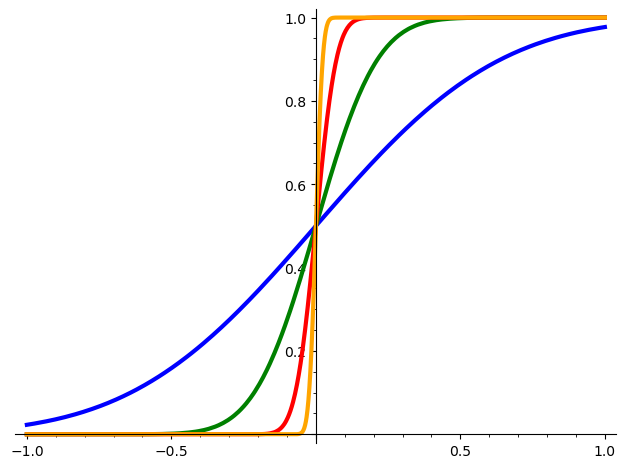
\includegraphics[width=0.5\textwidth]{graphics/gauss_cdfs}
\end{figure}

\begin{subsec}\label{all functions are measurable}
Let $\RR$ be equipped with its usual Lebesgue measure (or really any Borel measure $\mu$ on any space with a countable dense subset, such that for every countable set $Z$, $\mu(Z) = 0$).
Then any continuous function $\RR \to B$ pulls back open sets to open (hence Borel) sets and has separable image (since the image of $\QQ$ is dense in the image of $\RR$), hence is measurable by Theorem~\ref{characterization of measurable functions}.
Any pointwise limit of continuous functions is also measurable; for example any function with only a discrete set of discontinuities, or with only jump discontinuities.
A monotone function has only jump discontinuities, so is measurable. A similar argument applies for any left-continuous or right-continuous function.
And of course, we can modify any of the above functions on a countable set (or any null set!) to get another measurable function.
See Exercise~\ref{all functions are measurable exer} and Figure~\ref{Gauss convergence}.
\end{subsec}

\begin{subsec}
Which almost separably valued functions are nonmeasurable?
If $A \subseteq X$ is a nonmeasurable set then $1_{A}$ pulls back the Borel set $\{1\}$ to the nonmeasurable set $A$, so that $1_{A}$ is nonmeasurable.
An example of a nonmeasurable set is Vitali's set (Theorem~\ref{Vitali's set}).
\end{subsec}

\begin{example}\label{nonseparable function}
An example of a function which is not almost separably valued is given by Example~\ref{nonseparable space}.
Let $\delta$ be as in that example and let $f(x) = \delta_{x}$. Then for any uncountable $Y \subseteq \RR$, $f(Y)$ is an uncountable discrete set, so removing a null set cannot possibly help us here.
\end{example}

\begin{exercise}\label{all functions are measurable exer}
Prove the assertions in Example~\ref{all functions are measurable}.
\end{exercise}

\begin{definition}
Define the \dfn{Baire space} $B_{n}$ inductively: let $B_{0}$ be the space of continuous functions $[0, 1] \to \CC$, and let $B_{n+1}$ be the space of pointwise limits of functions in $B_{n}$.
If $f \in B_{n}$, we say that $f$ is \dfn{$n$-Baire}.

Unfortunately, there is another notion of Baire space, having to do with the Baire category theorem, which is not the same as the Baire space that we just defined.
\end{definition}

\begin{exercise}
Show that every Baire function is Borel.
(The converse is true if one allows for $\alpha$-Baire functions, $\alpha$ any countable ordinal, but you are not being asked to prove that.)
\end{exercise}

\begin{exercise}
Show that the derivative of a differentiable function is $1$-Baire.
Show that the function $1_{\QQ \cap [0, 1]}$ is $2$-Baire but not $1$-Baire.
\end{exercise}

\begin{exercise}
Find a function which is $3$-Baire but not $2$-Baire. More generally, find a function which is $(n+1)$-Baire but not $n$-Baire.
\end{exercise}

\section{Convergence of measurable functions}
We have already discussed two means by which measurable functions may converge to other measurable functions: pointwise and almost pointwise.
From this point onwards, pointwise convergence will be largely irrelevant; following our philosophy that null sets are important, almost pointwise will usually be the desired property.

\begin{subsec}
Throughout, we fix a complete measured space $(X, \Sigma, \mu)$ and a Banach space $B$.
\end{subsec}

\begin{definition}
A sequence of functions $f_{n}$ converge to a function $f$ \dfn{uniformly} if for every $\varepsilon > 0$ there is an $N$ such that for every $n > N$, $\sup ||f_{n} - f||_{B} < \varepsilon$.
\end{definition}

\begin{subsec}
Now, by analogy with the notion of a property holding ``almost everywhere'' (everywhere except a null set), we introduce the notion of a property holding \dfn{nearly everywhere}; that is, everywhere except a set of measure $\varepsilon > 0$. The property holds for arbitrarily small $\varepsilon$, but the parameters in the property (the $\delta$s, $N$s, and so on) may become arbitrarily ``bad'' as $\varepsilon \to 0$.
\end{subsec}

\begin{definition}
A sequence of functions $f_{n}: X \to B$ \dfn{converges nearly uniformly} to a function $f: X \to B$ if for every $\varepsilon > 0$ there is a set $E_{\varepsilon}$ such that $|\mu|(X \setminus E_{\varepsilon}) < \varepsilon$ and $f_{n} \to f$ uniformly on $E_{\varepsilon}$.
\end{definition}

\begin{figure}
\label{nearly uniform figure}
\caption{The sequence of functions $f_n(x) = x^n$ defined on $[0, 1]$ converges nearly uniformly, and hence almost everywhere, to $0$. Here $f_1$ is blue, $f_2$ is green, $f_4$ is red, and $f_8$ is orange. The defect near $1$ implies that they do not converge uniformly.}
\centering 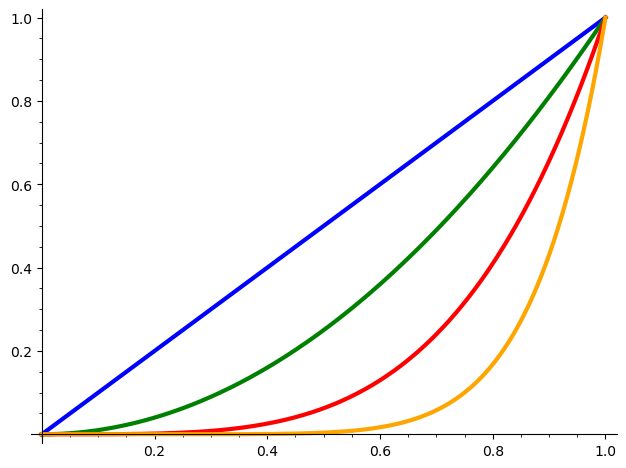
\includegraphics[width=0.5\textwidth]{graphics/nearly_uniform}
\end{figure}

\begin{subsec}
Thus $f_{n} \to f$ nearly uniformly iff for every $\varepsilon > 0$ there is a $E$ such that for every $\delta > 0$ there is an a $N$ such that $|\mu|(E) < \varepsilon$ and for every $n > N$, $\sup_{E} ||f_{n} - f||_{B} < \delta$.
Clearly a sequence which converges nearly uniformly converges almost pointwise; indeed, the sets $E_{\varepsilon}$ where the sequence fails to converge uniformly have a null intersection $E$, and if the sequence fails to converge pointwise at a point $x$, then $x \in E$.
In particular, the nearly uniform limit of a sequence of measurable functions is measurable.
See Figure \ref{nearly uniform figure} for an example of nearly uniform convergence which is not uniform.
\end{subsec}

\begin{lemma}
Suppose that $f_{n}: X \to B$ and $g_{n}: X \to B$, $f_{n} \to f$ and $g_{n} \to g$ nearly uniformly. Then the following limits also hold nearly uniformly:
\begin{enumerate}
\item $f_{n} + g_{n} \to f + g$.
\item For every $c \in \CC$, $cf_{n} \to cf$.
\item If $B = \CC$, $f_{n}g_{n} \to fg$.
\item $(x \mapsto ||f_{n}(x)||_{B}) \to (x \mapsto ||f(x)||_{B})$.
\item $\max(f_{n}, g_{n}) \to \max(f, g)$.
\item $\min(f_{n}, g_{n}) \to \min(f_{n}, g_{n})$.
\end{enumerate}
\end{lemma}
\begin{proof}
Routine and omitted.
\end{proof}

\begin{theorem}[Egorov]
Let $X$ be a finite measure space (thus $\mu(X) < \infty$) and suppose that $f_{n} \in M(X \to B)$ almost converge to $f$, and the $f_{n}$ are measurable.
Then $f_{n} \to f$ nearly uniformly.
\end{theorem}
\begin{proof}
After throwing away a harmless null set, we may assume that $f_{n} \to f$ pointwise. Now define
\[E_{m}^{n} = \{x \in X: \exists k \geq n(||f(x) - f_{k}(x)||_{B} \geq \frac{1}{m})\}.\]
Since $x \mapsto ||f(x) - f_{k}(x)||_{B}$ is measurable, by Theorem~\ref{characterization of measurable functions}, $E_{mn}$ is measurable.
Moreover, if $m$ is fixed, the $E_{m}^{n}$ shrink as $n$ increases and $\bigcap_{n} E_{mn} = \emptyset$, since $f_{n} \to f$.
By Lemma TODO, since $|\mu|(X) < \infty$, $\lim_{n} \mu(E_{m}^{n}) = 0$. So for every $\varepsilon > 0$ and every $m$ we may find $n(m)$ such that
\[\mu(E_{m}^{n(m)}) < \frac{\varepsilon}{2^{m}}.\]
Now let $F = E \setminus \bigcup_{m} E_{m}^{n(m)}$, so
\[\mu(E \setminus F) \leq \sum_{m=1}^{\infty} \mu(E_{m}^{n(m)}) < \varepsilon.\]
So it suffices to show that for every $\delta > 0$ there is a $N$ such that for every $n > N$, $\sup_{F} ||f_{n} - f||_{B} < \delta$.
Indeed, if $1/m < \delta$ and $N = n(m)$, then for every $x \in F$, $x \notin E_{N}^{m}$, so if $n > N$ then $||f(x) - f_{n}(x)||_{B} < \delta$.
\end{proof}

\begin{definition}
A sequence of functions $f_{n}: X \to B$ is said to be a \dfn{nearly uniform Cauchy sequence} if for every $\varepsilon > 0$ there is a measurable set $E_{\varepsilon}$ such that $\mu(X \setminus E_{\varepsilon}) < \varepsilon$ and for every $\delta > 0$ there is an $N$ such that for every $n_{1}, n_{2} > N$, $\sup ||f_{n_{1}} - f_{n_{2}}||_{B} < \delta$.
\end{definition}

\begin{subsec}
Since the hypothesis of being nearly uniform Cauchy is not altered if we change the functions $f_{n}$ on a null set, we can work with equivalence classes of functions (equivalent iff equal almost everywhere) rather than functions themselves. This will be important when we demand that the limit of a Cauchy sequence be unique; it will not be a unique function everywhere, but only almost everywhere.
\end{subsec}

\begin{lemma}\label{nearly uniform cauchy converges}
Let $f_{n} \in M(X \to B)$ be a nearly uniform Cauchy sequence. Then there is a unique $f \in M(X \to B)$ such that $f_{n} \to f$ nearly uniformly.
\end{lemma}
\begin{proof}
For every $m$ we can find $E_{m}$ such that $|\mu|(X \setminus E_{m}) < 1/m$ and $f_{n}$ is uniformly Cauchy on $E_{m}$. Let $E = \bigcup_{m} E_{m}$.
Then $|\mu|(X \setminus E) < 1/m$ for every $m$, so $|\mu|(X \setminus E) = 0$, and it is okay if we leave $f$ undefined on $X \setminus E$.
As for if $x \in E$, we can choose an $m$ such that $x \in E_{m}$. Since the $f_{n}$ are a nearly uniform Cauchy sequence, the $f_{n}(x)$ are a Cauchy sequence, which converge to some $y \in B$ since $B$ is a Banach space.
Therefore we may let $f(x) = y$.

Now the $f_{n} \to f$ nearly uniformly. In fact, for every $\varepsilon > 0$ we may take $m > 1/\varepsilon$ and let $E_{\varepsilon} = E_{m}$.
Then $f_{n} \to f$ uniformly on $E_{\varepsilon}$.

As for uniqueness, the $f_{n} \to f$ almost pointwise, and pointwise limits are unique (so that almost pointwise limits are unique almost everywhere). But $f$ was only defined up to measure zero, so this is no loss.
\end{proof}

\begin{definition}
Let $f_{n}: X \to B$ be a sequence of measurable functions, $f: X \to B$. We say that $f_{n}$ \dfn{converges in measure} to $f$ if for every $\varepsilon > 0$ the set
\[\lim_{n\to \infty} |\mu|(\{x \in X: ||f_{n}(x) - f(x)||_{B} > \varepsilon\}) = 0.\]
If $\mu$ is a probability measure, we instead say that $\mu$ \dfn{converges in probability}.
\end{definition}

\begin{subsec}
We sometimes abbreviate the set in the above definition as $\{||f_{n} - f||_{B} > \varepsilon\}$.
In other words, $f_{n} \to f$ in measure iff for every $\varepsilon > 0$ and every $\delta > 0$ there is an $N$ such that for every $n > N$,
\[|\mu|(\{||f_{n} - f||_{B} > \varepsilon\}) < \delta,\]
and collapsing quantifiers this happens iff for every $\varepsilon > 0$ there is an $N$ such that for every $n > N$,
\[|\mu|(\{||f_{n} - f||_{B} > \varepsilon\}) < \varepsilon.\]
\end{subsec}

\begin{subsec}
What is the intuition for convergence in measure?
Suppose that we are scientists running experiments in an attempt to compute the value of a function $f$.
As the number of test subjects $n$ goes to infinity, the experimental data $f_{n}$ should converge to $f$, but in what sense?
Let $X$ be the set of possible outcomes and $P(E)$ the probability that one of the outcomes in $E$ occurs, thus $P$ is a probablity measure. Then $P(\{||f_{n}(x) - f(x)||_{B} > \varepsilon\})$
is the probability that we got an experimental error of size at least $\varepsilon$; as $n \to \infty$, this probability becomes vanishingly small.
However, on the off-chance that an error of size at least $\varepsilon$ occurs, we have no control over how bad the error may be!
Thus $f_{n} \to f$ in probability and a priori we can prove no stronger.
\end{subsec}

\begin{lemma}\label{conv in measure is hausdorff}
If $f_{n} \to f$ in measure, then $f$ is unique almost everywhere, hence as an element of $M(X \to B)$.
\end{lemma}
\begin{proof}
Suppose that $f_{n} \to g$ in measure as well. Then for every $\varepsilon > 0$ and $n$,
\[\{||f - g||_{B} > \varepsilon\} \subseteq \{||f - f_{n}||_{B} > \varepsilon/2\} \cup \{||g - f_{n}||_{B}   > \varepsilon/2\}.\]
If $n$ is large enough, the right hand side has measure at most $\varepsilon$.
\end{proof}

\begin{definition}
Let $f_{n}: X \to B$ be a sequence of functions. We say that the $f_{n}$ are \dfn{Cauchy in measure} if for every $\varepsilon > 0$ there is a $N$ such that for every $n_{1}, n_{2} > N$,
\[|\mu|(\{||f_{n_{1}} - f_{n_{2}}||_{B} > \varepsilon\}) < \varepsilon.\]
\end{definition}

\begin{lemma}
Suppose that $f_{n}: X \to B$ and $g_{n}: X \to B$, $f_{n} \to f$ and $g_{n} \to g$ in measure. Then the following limits also hold in measure:
\begin{enumerate}
\item $f_{n} + g_{n} \to f + g$.
\item For every $c \in \CC$, $cf_{n} \to cf$.
\item If $B = \CC$, $f_{n}g_{n} \to fg$.
\item $(x \mapsto ||f_{n}(x)||_{B}) \to (x \mapsto ||f(x)||_{B})$.
\item $\max(f_{n}, g_{n}) \to \max(f, g)$.
\item $\min(f_{n}, g_{n}) \to \min(f, g)$.
\end{enumerate}
\end{lemma}
\begin{proof}
Routine and omitted.
\end{proof}

\begin{subsec}
How does convergence in measure relate to other modes of convergence?
It does not imply almost pointwise convergence --- imagine a sequence of functions racing back and forth along $[0, 1]$, their supports getting smaller with every time they turn around. TODO:\@ Draw a picture.
Nor does it follow from almost pointwise convergence on infinite measure sets --- just take $f_{n} = 1_{[n, n+1]}$ as a counterexample.
But convergence in measure is weaker than nearly uniform convergence, hence from almost pointwise convergence on finite measure sets. TODO:\@ Draw a diagram.
\end{subsec}

\begin{lemma}\label{nearly uniform implies in measure}
Suppose that $f_{n} \to f$ nearly uniformly; then $f_{n} \to f$ in measure.
\end{lemma}
\begin{proof}
Let $\varepsilon > 0$.
Then there is a set $E_{\varepsilon}$ on which $f_{n} \to f$ uniformly such that $\mu(X \setminus E_{\varepsilon}) < \varepsilon$, thus if $n$ is large enough $\sup_{E_{\varepsilon}} |f_{n} - f| < \varepsilon$, so $\{||f_{n} - f||_{B} > \varepsilon\} \subseteq X \setminus E_{\varepsilon}$ and hence $\mu(\{||f_{n} - f||_{B} > \varepsilon\}) < \varepsilon$.
So $f_{n} \to f$ in measure.
\end{proof}

\begin{corollary}
If $\mu(X) < \infty$ and $f_{n} \to f$ almost pointwise, then $f_{n} \to f$ in measure.
\end{corollary}
\begin{proof}
By Egorov's theorem and Lemma~\ref{nearly uniform implies in measure}.
\end{proof}

\begin{subsec}
We now come to a critical result which implies that Cauchyness in measure not only implies convergence in measure, but other modes of convergence as well.
This result has been called the \dfn{Riesz-Weyl theorem} or the \dfn{fundamental theorem of integration}.
\end{subsec}

\begin{theorem}[fundamental theorem of integration]
Suppose that $f_{n}$ is a Cauchy sequence in measure. Then there is a subsequence of $f_{n_{k}}$ and a unique $f \in M(X \to B)$ such that:
\begin{enumerate}
\item The $f_{n_{k}}$ are a nearly uniform Cauchy sequence.
\item $f_{n_{k}} \to f$ nearly uniformly.
\item $f_{n} \to f$ in measure.
\end{enumerate}
\end{theorem}
\begin{proof}
Let $n_{1} = 1$, and choose $n_{k+1} > n_{k}$ such that if $m_{1}, m_{2} \geq n_{k+1}$, then
\[|\mu|(\{||f_{m_{1}} - f_{m_{2}}||_{B} \geq 2^{-k}\}) < 2^{-k}.\]
Let $g_{k} = f_{n_{k}}$.
\begin{sublemma}
$g_{k}$ is nearly uniformly Cauchy.
\end{sublemma}
\begin{proof}
Let $\varepsilon > 0$ and choose $K$ so that $\sum_{k\geq K} 2^{-k} < \varepsilon$. Let
\[F = X \setminus \bigcup_{k \geq K} \{||g_{k} - g_{k+1}||_{B} > 2^{-k}\}.\]
Then $\mu(X \setminus F) < \varepsilon$.

Now let $\delta > 0$ and choose $N$ so large that $N \geq K$, $2^{1-N} < \delta$. Then if $j > \ell > N$, $x \in F$,
\begin{align*}
||g_{j}(x) - g_{\ell}(x)||_{B} &= ||g_{j}(x) - g_{j-1}(x) + g_{j-1}(x) - g_{j-2}(x) + \cdots + g_{\ell+1}(x) - g_{\ell}(x)||_{B}\\
&\leq \sum_{i=\ell}^{j-1} ||g_{i+1}(x) - g_{i}(x)||_{B}\\
&\leq \sum_{i=\ell}^{j-1} 2^{-i} < 2^{1-N} < \delta.
\end{align*}
Therefore the $g_{k}$ are a uniform Cauchy sequence on $F$ and hence nearly uniform on $X$.
\end{proof}
So by Lemma~\ref{nearly uniform cauchy converges}, there is an $f$ such that $\lim_{k} g_{k} = f$ nearly uniformly.
But then Lemma~\ref{nearly uniform implies in measure} implies that $\lim_{k} g_{k} = f$ in measure.
But
\begin{equation}\label{form1}\{||f - f_{n}(x)||_{B} > \varepsilon\} \subseteq \{||f - g_{k}||_{B} > \varepsilon/2\} \cup \{||f_{n} - g_{k}||_{B} > \varepsilon/2\},
\end{equation}
and the $g_{k}$ are a subsequence of the Cauchy-in-measure sequence $f_{n}$, hence the right hand side of (\ref{form1}) is $<\varepsilon$ if $n,k$ are large enough. So $f_{n} \to f$ in measure.
Uniqueness follows by Lemma~\ref{conv in measure is hausdorff}.
\end{proof}

\begin{corollary}
If $f_{n} \to f$ in measure, then there is a subsequence of $f_{n_{k}}$ such that $f_{n_{k}} \to f$ nearly uniformly.
\end{corollary}
\begin{proof}
The $f_{n}$ are Cauchy in measure, so the fundamental theorem of integration implies that there is a subsequence that is nearly uniformly Cauchy.
Uniqueness of a nearly uniform limit implies that the subsequence must converge to $f$.
\end{proof}

\begin{exercise}
Find an example which shows that the hypothesis of finite measure in Egorov's theorem cannot be omitted.
\end{exercise}

\section{Regularity of measurable functions}
Before we define the integral, we pause to use Egorov's theorem to prove a partial converse to the theorem which said that every continuous function was measurable.
Of course not every measurable function is continuous (most measure spaces don't even come with a topology, but also, any familiar discontinuous function on $\RR$ will be measurable), but we will do the best that we can this section.

\begin{subsec}
Throughout this section, fix a locally compact Hausdorff space $X$. If the reader is not familiar with such notions, they can take $X = \RR^{c}$.
\end{subsec}

\begin{subsec}
Recall that a function $f: \RR^{c} \to \CC^{d}$ is \dfn{smooth} if for every point $x$ and every vector of natural numbers $(k_{1}, \dots, k_{c})$, the partial derivative
\[\partial_{1}^{k_{1}} \partial_{2}^{k_{2}} \cdots \partial_{c}^{k_{c}} f(x)\]
exists; here $\partial_{i}^{k_{i}}$ is the operator that takes a function to its $k_{i}$th partial derivative along its $i$th basis vector.
Clearly every smooth function is differentiable and hence continuous.
\end{subsec}

\begin{lemma}[Urysohn]
Let $K_{0},K_{1} \subseteq X$ be disjoint closed sets. Then there is a continuous function $f: X \to [0, 1]$ such that $f|K_{0} = 0$ and $f|K_{1} = 1$.
Moreover, if $X = \RR^{c}$, we can even assume that $f$ is smooth.
\end{lemma}

\begin{subsec}
We refer the reader to the appendix for the proof of Urysohn's lemma.
We will also need the fact that every compact subset of a Hausdorff space is closed.
\end{subsec}

\begin{subsec}
Now the open sets of $X$ generate a topology, namely the Borel $\sigma$-algebra of $X$. Therefore $X$ is a measurable space in a natural way.
By a \dfn{Borel measure} on $X$ we mean a measure defined on the Borel $\sigma$-algebra of $X$.
\end{subsec}

\begin{lemma}
Every continuous function is measurable with respect to the Borel $\sigma$-algebra.
\end{lemma}
\begin{proof}
Let $f: X \to B$ be continuous; then the $f$-preimage of an open set is open, hence Borel, hence measurable.
We now appeal to Theorem~\ref{characterization of measurable functions}.
\end{proof}

\begin{definition}
View $X$ as a complete measured space $(X, \Sigma, \mu)$, where $\mu$ is a Borel measure and $\Sigma$ is the $\sigma$-algebra of $\mu$-measurable sets (so that $\Sigma$ is generated by the Borel sets and $\mu$-null sets).
Let $f: X \to B$ be a function.
We say that $f$ is a \dfn{nearly continuous function} if for every $\varepsilon > 0$ there is a set $E$ such that $\mu(X \setminus E) < \varepsilon$ and $f|E$ is continuous.
\end{definition}

\begin{subsec}
You should check that your favorite discontinuous function (that isn't the indicator function of the Vitali set) is nearly continuous.
For example the function $x \mapsto 1/x$ is nearly continuous because if we discard a small neighborhood of $0$, then it is continuous.
\end{subsec}

\begin{subsec}
Throughout the rest of the section, we fix a positive Radon measure $\mu$ on $X$, and take its completion, so if $\Sigma$ denotes the $\sigma$-algebra generated by Borel sets and $\mu$-null sets, then $(X, \Sigma, \mu)$ is a complete measured space, which we also denote by $X$.
Thus $X$ is equipped with a topology, a $\sigma$-algebra, and a measure; so $X$ is a lot like the real line $\RR$, and when we refer to measurable functions, nearly continuous functions, and so on, we do so with respect to $\Sigma$.
\end{subsec}

\begin{lemma}\label{smooth functions are pointwise dense}
If $f: X \to \CC^{d}$ is a measurable function, then there is a sequence of continuous functions $f_{n}: X \to \CC^{d}$ such that $f_{n} \to f$ almost pointwise.
If $X = \RR^{c}$ then we can even take the $f_{n}$ to be smooth.
\end{lemma}
\begin{proof}
We first check this when $f$ is the indicator function of a compact set $K$.
By outer regularity, for every $n$ there is an open set $U_{n} \supseteq K$ such that $\mu(U_{n} \setminus K) < 1/n$, and after taking intersections we can assume that $U_{n} \supseteq U_{n+1}$.
The complement $X \setminus U_{n}$ is closed, so by Urysohn's lemma there is a continuous function $f_{n}: X \to [0, 1]$, smooth if $X = \RR^{c}$, such that $f_{n}|K = 1$ and $f_{n}|(X \setminus U_{n}) = 0$.
Now $f_{n} \to f$ almost pointwise. Indeed, if $x \in K$, then for every $n$, $f_{n}(x) = 1$; otherwise, unless $x$ is in $\bigcap_{n} U_{n} \setminus K$, which is a null set, there is an $N$ such that $x \notin U_{N}$, and hence for every $n > N$, $x \notin U_{n}$, so $f_{n}(x) = 0$.
TODO:\@ Draw a picture.

We now check when $f$ is the indicator function of an open set $U$.
By inner regularity, there is a sequence of compact sets $K_{m}$ such that $K_{m} \subseteq K_{m+1}$ and $\mu(U \setminus K_{m}) < 1/m$.
In particular, $\lim_{m} 1_{K_{m}} = 1_{U}$ almost pointwise.
Now there are sequences of continuous functions (smooth if $X = \RR^{c}$) $f_{n}^{m}: X \to [0, 1]$ such that $\lim_{n} f_{n}^{m} = 1_{K_{m}}$ almost pointwise, thus
\[|f_{n}^{n}(x) - 1_{U}(x)| \leq |f_{n}^{n}(x) - 1_{K_{n}}(x)| + |1_{K_{n}}(x) - 1_{U}(x)|.\]
The right-hand side vanishes as $n \to \infty$ so $f_{n}^{n} \to 1_{U}$ almost pointwise.
TODO:\@ Draw a picture.

A similar argument applies when $f$ is the indicator function of a Borel set $W$.
Indeed, by outer regularity, there is a sequence of open sets $U_{m}$ such that $U_{m} \supseteq K_{m+1}$, $\mu(U_{m} \setminus W) < 1/m$.
We can find a sequence of continuous (smooth?) functions $f_{n}^{m}: X \to [0, 1]$ such that $\lim_{n} f_{n}^{m} = 1_{U_{m}}$ almost pointwise, and $\lim_{m} 1_{U_{m}} = 1_{W}$ almost pointwise, so $f_{n}^{n} \to 1_{W}$ almost pointwise.

If $f$ is the indicator function of a measurable set, then we can modify $f$ on a null set and replace it with the indicator function of a Borel set.

If $f \in \Simp(X \to \CC)$, then $f$ is a linear combination of indicator functions of measurable sets $f_{1}, \dots, f_{n}$, so we can find sequences approximating each of the summands $f_{i}$ and use linearity.

If $f$ is an arbitrary measurable function $X \to \CC$, we can approximate $f$ by simple functions.

If $f$ is a vector of measurable functions $X \to \CC^{d}$, we can approximate each of the components of $f$ by continuous (smooth?) functions.
\end{proof}

\begin{theorem}[Luzin]
If $\mu(X) < \infty$, then a function $f: X \to \CC^{d}$ is measurable iff $f$ is nearly continuous.
\end{theorem}
\begin{proof}
If $f$ is nearly continuous, then for every $\varepsilon > 0$ we can find a set $E_{\varepsilon}$ on which $f$ is continuous, hence measurable, and $\mu(X \setminus E_{\varepsilon}) < \varepsilon$.
Taking their union, we conclude that $f$ is measurable at almost every point of $X$, and hence everywhere on $X$.
Note that this direction was already valid for any Borel measure and any Banach space codomain.

Conversely, suppose that $f$ is measurable.
By Lemma~\ref{smooth functions are pointwise dense}, we can find a sequence of continuous (or even smooth) functions $f_{n}$ with $f_{n} \to f$ almost pointwise, and hence nearly uniformly by Egorov's theorem.
The uniform limit of a sequence of functions is continuous, so the nearly uniform limit is nearly continuous.
\end{proof}

\begin{exercise}
Show that there exists a measurable function on $\RR^{d}$ which is not nearly smooth.
\end{exercise}

\begin{exercise}
Let $\mu$ be a $\sigma$-finite positive Radon measure on $\RR^{d}$.
Show that for every Borel set $A$ such that $\mu(A) > 0$, there is an $R > 0$ such that $0 < \mu(B(0, R) \cap A) < \infty$.
Since this is in particular true for Lebesgue measure, it is often no loss of generality to suppose that the sets one is working with have finite Lebesgue measure.
\end{exercise}

\begin{exercise}
Let $\mu$ be Lebesgue measure on $\RR$.
Show that there is a Borel set $A \subseteq [0, 1]$ such that for every open interval $U \subseteq [0, 1]$, $0 < \mu(A \cap U) < \mu(U)$.
(Hint: Start with a fat Cantor set, c.f. Exercise~\ref{fat cat}, and then put more fat Cantor sets in the leftover intervals, but be careful.)
\end{exercise}

\begin{exercise}
Let $\mu$ be Lebesgue measure on $\RR$.
Let $A \subseteq \RR$ be a Borel set such that $\mu(A) > 0$.
Show that for every $\varepsilon > 0$ there is an open interval $U$ such that $\mu(U \cap A) > (1 - \varepsilon)\mu(U)$.
(Hint: Use the pigeonhole principle.)
\end{exercise}

\begin{exercise}\label{steinhaus}
Prove \dfn{Steinhaus' theorem}: Let $A$ be a Borel subset of $\RR$ with positive Lebesgue measure. Then the set $\{x - y: (x, y) \in A^{2}\}$ contains an open set $U$ such that $0 \in U$.
\end{exercise}

\begin{exercise}
Let $G \subset \RR$ be a proper subgroup of $\RR$ under addition.
Show that if $G$ is Borel then $G$ is null.
(Hint: use Exercise~\ref{steinhaus}, Steinhaus' theorem).
\end{exercise}


\section{Integration of simple functions}
We are ready to define the integral, at least for simple functions.

\begin{subsec}
A priori, our intuitive definition of integration as ``the net signed area under the graph'' is problematic.
Consider the function $f = 1_{[0, \infty)} - 1_{(-\infty, 0]}$. What is the net signed area under the graph of $f$? Well, to the left of $0$, it is $-\infty$, and to the right it is $+\infty$, so we run into our usual pesky foe, $\infty - \infty$.
To put off this problem for now, we dodge the issue by declaring that we will for now only try to integrate functions whose integrals will be finite.
\end{subsec}

\begin{subsec}
For the rest of the chapter, fix a measure $\mu$, either valued in $\CC$ (which is a one-dimensional Banach space) or $(-\infty, \infty]$.
The reason that we do not allow $\mu$ to be more generally vector-valued is that we need to be able to multiply elements of the Banach space $B$ by $\mu(E)$.
\end{subsec}

\begin{definition}
An \dfn{integrable simple function} is a function $f \in \Simp(X \to B)$ such that for every nonzero $b$ in the image of $f$, $f^{-1}(b)$ has finite measure.
We denote the set of integrable simple functions by $\ISF(X \to B)$.
\end{definition}

\begin{subsec}
We want the integral to be, at first, a linear map $\ISF(X \to B) \to B$.
To motivate it, let's suppose that $B = \CC$, $X = \RR$, $\mu$ is Lebesgue measure, and $E$ is an interval. Then $\int_{-\infty}^{\infty} 1_{E}$ had better be the area of the rectangle $E \times [0, 1]$ (TODO draw a picture), hence $\int_{-\infty}^{\infty} 1_{E} = \mu(E)$. In order for linearity to hold, if $c \in \CC$, we must then have $\int_{-\infty}^{\infty} c1_{E} = c\mu(E)$.
\end{subsec}

\begin{subsec}
For every integrable simple function $f$, $f$ can be written in terms of the indicator functions in a unique way; namely, if $\{b_{1}, \dots, b_{n}\}$ is the image of $f$,
\begin{equation}\label{canonical ISF rep}
f(x) = \sum_{i=1}^{n} b_{i}1_{f^{-1}(b_{i})}(x).
\end{equation}
In particular, the indicator functions span $\ISF(X \to \CC)$.
\end{subsec}

\begin{definition}
We call (\ref{canonical ISF rep}) the \dfn{canonical representation} of the integrable simple function $f$ with image $\{b_{1}, \dots, b_{n}\}$.
\end{definition}

\begin{definition}
Let $f \in \ISF(X \to B)$ and suppose that (\ref{canonical ISF rep}) is the canonical representation of $f$. Let $E$ be a measurable set. We define the \dfn{integral} of $f$ to be
\[\int_{E} f~d\mu = \sum_{i=1}^{n} b_{i}\mu(f^{-1}(b_{i}) \cap E).\]
\end{definition}

\begin{subsec}
We will occasionally write $\int f$ or similar to mean $\int_{X} f~d\mu$, but only when $X$ and $\mu$ are understood. If we need a dummy variable, we may write $\int_{E} f(x)~d\mu(x)$, and if $\mu$ is understood we may even write $\int_{E} f(x)~dx$. If $E$ is an interval $[a, b]$, we may write $\int_{a}^{b}$ to mean $\int_{E}$.
For example, once we will have adequately defined integration,
\[\int_{0}^{2\pi} \sin x~dx = 0\]
as one would expect.
\end{subsec}

\begin{lemma}\label{properties of ISF integral}
Let $f,g \in \ISF(X \to B)$. Then:
\begin{enumerate}
\item \dfn{Linearity}: For every $c \in \CC$,
\[\int_{X} cf + g~d\mu = c\int_{X} f ~d\mu + \int_{X} g~d\mu.\]
\item The \dfn{triangle inequality}:
\[\left|\left|\int f(x) ~d\mu(x)\right|\right|_{B} \leq \int ||f(x)||_{B} ~d|\mu|(x).\]
\item The \dfn{change-of-variables formula}: Let $(Y, \nu)$ be a measured space. Suppose that $h: Y \to X$ is a measurable map and $\mu$ is the pushforward measure $\mu = h_{*}\nu$. Then
\[\int_{X} f~d\mu = \int_{Y} f \circ h~d\nu.\]
\item If $B = \RR$ and $f \leq g$, then $\int f \leq \int g$.
\item If $E,F$ are disjoint measurable sets, then
\[\int_{E \cup F} f = \int_{E} f + \int_{F} f.\]
\item If $E \subseteq F$ are measurable sets, $B = \RR$, and $\mu$ is a nonnegative measure, then
\[\int_{E} f~d\mu \leq \int_{F} f~d\mu.\]
\item $\int ||f(x)||_{B} ~d|\mu|(x) = 0$ if and only if $f = 0$ almost everywhere.
\end{enumerate}
\end{lemma}
\begin{proof}
See Exercise~\ref{integral props exer 1}.
\end{proof}

\begin{subsec}
We want to extend the integral from $\ISF(X \to B)$ to the space $M(X \to B)$ of all measurable functions.
But we cannot merely define $\int f = \lim_{n} f_{n}$, where the $f_{n}$ are simple functions that converge to $f$.
Indeed, if $f_{n} = 1_{[n, n+1]}$ then $f_{n} \to 0$ pointwise, but $\lim_{n} \int f_{n} = 1$, and we certainly do not want $\int 0 = 1$!
We need another notion of convergence, which will turn out to be closely related to convergence in measure.
\end{subsec}

\begin{definition}
Given $f \in \ISF(X \to B)$, let
\begin{equation}\label{L1 norm dfn}
||f||_{1} = \int_{X} ||f(x)||_{B} ~d|\mu|(x).
\end{equation}
One calls $||f||_{1}$ the \dfn{$L^{1}$-norm} of $f$.
\end{definition}

\begin{subsec}
As the reader should check, the $L^{1}$ norm is a seminorm. See Exercise~\ref{L1 norm exer}.
Now when we say that $f_{n} \to f$ in $L^{1}$, we mean that $||f_{n} - f||_{1} \to 0$. Similarly if we say that the $f_{n}$ are Cauchy in $L^{1}$, we mean that $||f_{n} - f_{m}||_{1} \to 0$.
\end{subsec}

\begin{subsec}
It is natural to want to extend the $L^{1}$ norm to the completion of the space $\ISF(X \to B)$, on which it will actually be a norm.
(See Theorem~\ref{completion exists} for more on that.)
\end{subsec}

\begin{definition}
The completion of $\ISF(X \to B)$ is known as $L^{1}(X \to B)$.
\end{definition}

\begin{subsec}
Formally, $L^{1}(X \to B)$ consists of Cauchy sequences of simple functions modulo Cauchy equivalence.
We will define the integral as a linear map $L^{1}(X \to B) \to B$:
\end{subsec}

\begin{definition}\label{definition of integral}
Let $f \in L^{1}(X \to B)$ and suppose that $E$ is a measurable set.
Choose a Cauchy sequence of $f_{n} \in \ISF(X \to B)$ such that $f_{n} \to f$ in $L^{1}$.
We define the \dfn{integral} of $f$ to be
\[\int_{E} f~d\mu = \lim_{n \to \infty} \int_{E} f_{n}~d\mu.\]
\end{definition}

\begin{subsec}
Let's check that Definition~\ref{definition of integral} makes sense. When we say that $f_{n} \to f$ in $L^{1}$, we mean that $f$ is the equivalence class of the Cauchy sequence ${(f_{n})}_{n}$.
So if there was another Cauchy sequence ${(g_{n})}_{n}$ with $g_{n} \to f$ in $L^{1}$,
\begin{align*}\left|\left|\lim_{n \to \infty} \int_{E} g_{n} - f_{n} ~d\mu\right|\right| &\leq \lim_{n \to \infty} \int_{E} ||g_{n}(x) - f_{n}(x)||_{B} ~d|\mu|(x)\\&
\leq \lim_{n \to \infty} \int_{X} ||g_{n}(x) - f_{n}(x)||_{B} ~d|\mu|(x)
\\& = \lim_{n \to \infty} ||g_{n} - f_{n}||_{1} = 0,
\end{align*}
the last equality following because the $g_{n}$ and the $f_{n}$ are Cauchy equivalent.
Therefore the choice of Cauchy sequence in Lemma~\ref{definition of integral} is immaterial, and any choice will return the same integral.
As a consequence, the $L^{1}$ norm extends to all of $L^{1}(X \to B)$ by the equation (\ref{L1 norm dfn}).
\end{subsec}

\begin{lemma}\label{properties of ISF integral 2}
The conclusion of Lemma~\ref{properties of ISF integral} holds for any $f,g \in L^{1}(X \to B)$, not just $f,g \in \ISF(X \to B)$.
\end{lemma}
\begin{proof}
Left as Exercise~\ref{integral props exer 2}.
\end{proof}

\begin{exercise}\label{integral props exer 1}
Prove Lemma~\ref{properties of ISF integral}.
\end{exercise}

\begin{exercise}\label{L1 norm exer}
Show that the $L^{1}$-norm is a seminorm on $\ISF$, and that $||f||_{1} = 0$ iff $f = 0$ almost everywhere.
\end{exercise}

\begin{exercise}\label{integral props exer 2}
Prove Lemma~\ref{properties of ISF integral 2}.
\end{exercise}

\begin{exercise}
Let $A = \{1, \dots, d\}$ with counting measure. Therefore \emph{every} function $A \to \RR$ is an integrable simple function, and we can identify $f \in \ISF(A \to \RR)$ with the vector $(f(1), \dots, f(d))$.
So we can identify $\ISF(A \to \RR)$ with $\RR^{d}$.
Show that the topology induced by the $L^{1}$-norm on $\RR^{d}$ is the usual euclidean topology on $\RR^{d}$.
What is the unit ball in the $L^{1}$-norm shaped like?
\end{exercise}

\section{The integral in general}
The conclusion of the previous section, wherein we treated the integral on $L^{1}(X \to B)$, was really quite silly.
We want to integrate functions, not equivalence classes of Cauchy sequences of simple functions.
This is analogous to how we want to study real numbers, not equivalence classes of Cauchy sequences of rational numbers.
We need some sort of isomorphism which sends functions to members of $L^{1}$.

\begin{theorem}[fundamental theorem of integration, part II]
Suppose that $f_{n} \to f$ in $L^{1}$. Then there is a function $f'$ such that $f_{n} \to f'$ in measure and there is a subsequence of $f_{n_{k}}$ such that $f_{n_{k}} \to f'$ nearly uniformly, and hence almost pointwise.
\end{theorem}
\begin{proof}
We have to show that the $f_{n}$ are Cauchy in measure; the other claims follow from the first part of the fundamental theorem of integration.

To see that the $f_{n}$ are Cauchy in measure, we reason by contraposition, so suppose that we are given a subsequence $f_{k_{n}}$ and a $\varepsilon > 0$ such that for every $n,m$,
\[\{||f_{k_{m}} - f_{k_{n}}||_{B} > \varepsilon\} > \varepsilon.\]
Then
\begin{align*}
||f_{k_{m}} - f_{k_{n}}||_{1} &= \int_{X} ||f_{k_{m}}(x) f_{k_{n}}(x)||_{B}~d\mu(x)\\
&\geq \int_{\{||f_{k_{m}} - f_{k_{n}}||_{B} > \varepsilon\}} ||f_{k_{m}}(x) f_{k_{n}}(x)||_{B}~d\mu(x)\\
&\geq \int_{\{||f_{k_{m}} - f_{k_{n}}||_{B} > \varepsilon\}} \varepsilon ~d\mu(x)\\
&= \varepsilon \int_{\{||f_{k_{m}} - f_{k_{n}}||_{B} > \varepsilon\}} ~d\mu(x)\\
&= \varepsilon |\mu|(\{||f_{k_{m}} - f_{k_{n}}||_{B} > \varepsilon\}) > \varepsilon^{2} > 0.
\end{align*}
Therefore the $f_{n}$ are not Cauchy in $L^{1}$, so they do not converge in $L^{1}$.
\end{proof}

\begin{subsec}
Now if $f_{n} \to f$ in $L^{1}$ and $f_{n} \to f'$ in measure, then it is tempting to identify $f'$ with $f$, but we need to check that the choice of $L^{1}$ Cauchy sequence does not matter.
\end{subsec}

\begin{theorem}[fundamental theorem of integration, part III]
Suppose that $f_{n} \to f$ in $L^{1}$ and $f_{n} \to f'$ in measure.
If $g_{n} \to f$ in $L^{1}$, then $g_{n} \to f'$ in measure.
Conversely, if the $g_{n}$ are Cauchy in $L^{1}$ and $g_{n} \to f'$ in measure, then $g_{n} \to f$ in $L^{1}$.
\end{theorem}
\begin{proof}
Suppose that $g_{n} \to f$ in $L^{1}$.
Then the sequence $(f_{1}, g_{1}, f_{2}, g_{2}, \dots)$ is Cauchy in $L^{1}$, hence Cauchy in measure; but it has a subsequence which converges in measure to $f'$ in measure, so the mother sequence must also converge in measure to $f'$, and hence every subsequence, including the $g_{n}$, must converge in measure to $f'$.

As for the converse, we use part I of the fundamental theorem of integration to show that there are subsequences $f_{n_{k}}, g_{n_{k}}$ which converge nearly uniformly to $f'$, and are Cauchy in $L^{1}$.
Let $h_{k} = f_{n_{k}} - g_{n_{k}}$. Then the $h_{k}$ is Cauchy in $L^{1}$, converge nearly uniformly to $0$, and if $h_{k} \to 0$ in $L^{1}$ then the $f_{n_{k}}$ and $g_{n_{k}}$ are Cauchy equivalent.
\begin{lemma}
$h_{k} \to 0$ in $L^{1}$.
\end{lemma}
\begin{proof}
Let $\varepsilon > 0$, and choose $N$ so that if $n_{1}, n_{2} \geq N$ then $||h_{n} - h_{m}||_{1} < \varepsilon$. We claim that $||h_{N}||_{1} \lesssim \varepsilon$ where the implied constant only depends on the sequence and not on the index $N$, so that if $n > N$ then
\[||h_{n}||_{1} \leq ||h_{n} - h_{N}||_{1} + ||h_{N}||_{1} \lesssim \varepsilon.\]
But $h_{N} \in \ISF(X \to B)$, so the carrier $E$ of $h_{N}$ satisfies $\mu(E) < \infty$, and $h_{N}$ is bounded, thus $||h_{N}(x)|| \lesssim 1$, where the implied constant does not depend on $x$ or the index $N$, but only on the sequence.

Since $h_{n} \to 0$ nearly uniformly, there is a measurable set $F \subseteq E$ such that $|\mu|(E \setminus F) < \varepsilon$ and $h_{n} \to 0$ uniformly on $F$. Therefore
\[\int_{E \setminus F} ||h_{n}(x)||_{B} ~d|\mu|(x) \lesssim \int_{E \setminus F} ~|\mu|(x) = |\mu|(E \setminus F) < \varepsilon.\]
Meanwhile, if $N$ is large enough, then $||h_{N}(x)||_{B} < \varepsilon$ for every $x \in F$,
\[\int_{F} ||h_{N}(x)||_{B}~d|\mu|(x) < \varepsilon |\mu|(F) \leq \varepsilon |\mu|(E).\]
So
\[||h_{N}||_{1} = \int_{X} ||h_{N}(x)||_{B} ~d|\mu|(x) \lesssim \varepsilon\]
which was to be shown.
\end{proof}

Hence the $f_{n_{k}}$ and $g_{n_{k}}$ are Cauchy equivalent.
Since the mother sequences $f_{n}$ and $g_{n}$ are Cauchy, if they have subsequences that are Cauchy equivalent, then the $f_{n}$ and $g_{n}$ are Cauchy equivalent, so since $f_{n} \to f$ in $L^{1}$, $g_{n} \to f$ in $L^{1}$.
\end{proof}

\begin{subsec}
Summarizing, if $f \in L^{1}$, then there is an $f' \in M$ with the following property: for every $L^{1}$ Cauchy sequence $f_{n} \in \ISF$ such that $f_{n} \to f$ in $L^{1}$, such that $f_{n} \to f'$ in measure, nearly uniformly along a subsequence, and almost pointwise along a subsequence.
Moreover, $L^{1}$ is the completion of $\ISF$, so such a $L^{1}$ Cauchy sequence must exist.
\end{subsec}

\begin{corollary}
Let $f \in M$, and suppose the $f_{n} \in \ISF$ are an $L^{1}$ Cauchy sequence. Then the following are equivalent:
\begin{enumerate}
\item $f_{n} \to f$ in measure.
\item $f_{n} \to f$ nearly uniformly.
\item $f_{n} \to f$ almost everywhere.
\end{enumerate}
\end{corollary}
\begin{proof}
That $1$ implies $2$ implies $3$ is the content of the fundamental theorem of integration.
Now if $f_{n} \to f$ almost everywhere, Egorov's theorem furnishes a subsequence $f_{n_{k}}$ which converges to $f$ nearly uniformly, hence in measure.
But the $f_{n}$ are Cauchy in $L^{1}$, hence in measure; if the mother sequence is Cauchy and a subsequence converges, the mother sequence converges, so $f_{n} \to f$ in measure.
\end{proof}

\begin{subsec}
Elements of $M$ are functions up to the equivalence relation of being equal almost everywhere.
That is,
\[M = \frac{\mathcal M}{\mathcal N}\]
where $\mathcal M$ is the space of all measurable functions and $\mathcal N$ is the space of measurable functions which are zero almost everywhere.
Therefore if $f_{n} \to f$ in $L^{1}$ and $f_{n} \to f'$ in measure (equivalently, nearly uniformly, or almost everywhere), we can actually identify $f$ with $f'$ and think of $f'$ as a ``function'' by choosing a version of $f'$.
Henceforth we will not make a distinction between elements of $L^{1}$, elements $f$ of $M$ which admit an $L^{1}$ Cauchy sequence of simple functions which converge to $f$ in measure, and versions of $f$.
Therefore we are (finally!) ready to define the integral in general.
\end{subsec}

\begin{definition}
Let $f \in M(X \to B)$, and suppose that there is a $L^{1}$ Cauchy sequence $f_{n} \in \ISF(X \to B)$ such that $f_{n} \to f$ in measure. Then we say that $f \in L^{1}(X \to B)$, define for any measurable set $E$ the \dfn{integral}
\[\int_{E} f ~d\mu = \lim_{n \to \infty} \int_{E} f_{n}~d\mu,\]
and the \dfn{$L^{1}$ norm}
\[||f||_{1} = \int_{X} ||f(x)||_{B} ~d|\mu|(x).\]
If the integral $\int_{X} f~d\mu$ exists, we say that $f$ is \dfn{integrable} or \dfn{summable}.
\end{definition}

\begin{theorem}
Let $f,g \in L^{1}(X \to B)$. Then:
\begin{enumerate}
\item \dfn{Linearity}: For every $c \in \CC$,
\[\int_{X} cf + g~d\mu = c\int_{X} f ~d\mu + \int_{X} g~d\mu.\]
\item The \dfn{triangle inequality}:
\[\left|\left|\int_{X} f(x) ~d\mu(x)\right|\right|_{B} \leq \int_{X} ||f(x)||_{B}~d|\mu|(x).\]
\item The \dfn{change-of-variables formula}: Let $(Y, \nu)$ be a measured space. Suppose that $h: Y \to X$ is a measurable map and $\mu$ is the pushforward measure $\mu = h_{*}\nu$. Then
\[\int_{X} f~d\mu = \int_{Y} f \circ h~d\nu.\]
\item If $B = \RR$ and $f \leq g$, then $\int f \leq \int g$.
\item If $E,F$ are disjoint measurable sets, then
\[\int_{E \cup F} f = \int_{E} f + \int_{F} f.\]
\item If $E \subseteq F$ are measurable sets, $B = \RR$, and $\mu$ is a nonnegative measure, then
\[\int_{E} f~d\mu \leq \int_{F} f~d\mu.\]
\item $\int ||f(x)||_{B} ~d\mu(x) = 0$ if and only if $f = 0$ almost everywhere.
\end{enumerate}
\end{theorem}
\begin{proof}
This follows from the previous version of the theorem by density in $L^{1}$.
\end{proof}

\begin{subsec}
We can extend the definition of the integral even further.
If $f \in M(X \to B)$ has a nonnegative version, we write $f \geq 0$.
\end{subsec}

\begin{definition}
Let $f \in M(X \to B)$, and assume that $f \geq 0$. Let $E$ be a measurable set. If for every $L^{1}$ Cauchy sequence $f_{n} \in \ISF(X \to B)$, $f_{n}$ does not converge to $1_{E} f$ in measure, then we write
\[\int_{X} f ~d\mu = \infty\]
provided that $\mu$ is a nonnegative measure.
\end{definition}

\begin{subsec}
Now if $f \in M(X \to \CC)$, we can write $f = f_{a} + if_{b}$ where $f_{a}, f_{b}$ are real-valued, and $\int f = \int f_{a} + i\int f_{b}$.
So integration of complex-valued functions reduces to integration of real-valued functions. Moreover, if $f$ is real-valued then we can write $f = f_+ - f_-$ where $f_{\pm} \geq 0$. So $\int f = \int f_+ - \int f_-$.
This makes sense even if one (but not both!) of the $\int f_{\pm}$ is infinite.
Thus the only measurable functions which cannot be integrated are those whose integrals would be $\infty - \infty$.
That's a far cry from the Riemann integral, whose definition was quite restricted!
\end{subsec}

\begin{subsec}
While in practice we identify functions which are equal almost everywhere, sometimes it is convenient to work with functions, rather than their equivalence classes.
Recall that $\mathcal M$ is the space of measurable functions; analogously we let $\mathcal L^{1}$ denote the space of functions whose equivalence classes are in $L^{1}$. If $f \in \mathcal L^{1}$, we let $[f]$ denote the equivalence class of $f$ and define
\[\int_{E} f ~d\mu = \int_{E} [f]~d\mu.\]
This definition then extends to those elements of $\mathcal M$ whose integral is not $\infty - \infty$.
Notice that $||\cdot||_{1}$ is a seminorm on $\mathcal L^{1}$, and a norm on $L^{1}$.
\end{subsec}

\begin{subsec}
Let us now recast the above in the language of probability theory.
\end{subsec}

\begin{definition}
Let $(\Omega, P)$ be a probability space.
Let $X$ be a random variable of type $B$ on $\Omega$.
The \dfn{expected value} of $X$ is
\[EX = \int_{\Omega} X~dP\]
provided that $X \in L^{1}$.
If in addition $X^{2} \in L^{1}$ and $B = \RR$, then the \dfn{variance} of $X$ is
\[\Var X = E{((X - EX)}^{2}).\]
The \dfn{standard deviation} of $X$ is $\sqrt{\Var X}$.
\end{definition}

\begin{exercise}\label{Chebyshev}
Let $\mu$ be a positive measure.
Prove \dfn{Chebyshev's inequality}, which says that if $f \in M$, then for any $t > 0$ and $p > 0$,
\[\mu(||f(x)||_{B} \geq t) \leq t^{-p} \int_{||f||_{B} \geq t} ||f||_{B}^{p}~d\mu.\]
Here $||f||_{B} \geq t$ is the set $\{x \in X: ||f(x)||_{B} \geq t\}$.
\end{exercise}

\begin{exercise}
Let $\delta_{x}$ be the Dirac measure at $x \in \RR$, as in Exercise~\ref{Dirac measure}.
Show that every function $f: \RR \to B$ is Dirac measurable and compute the integral $\int_{\RR} f~d\delta_{x}$.
\end{exercise}

\begin{exercise}
Let $X$ be a random variable of type $\RR$. Show that
\[\Var X = E(X^{2}) - {(EX)}^{2} \geq 0\]
with equality iff $X$ is almost surely constant, as long as the definition of $\Var X$ makes sense.
\end{exercise}

\begin{exercise}\label{integrating a distribution}
Let $X$ be a random variable of type $\RR$ and distribution $\mu$. Show that
\[EX = \int_{-\infty}^{\infty} x ~d\mu(x)\]
as long as the definition of $EX$ makes sense.
\end{exercise}
